\documentclass[12pt, a4paper]{article}
\usepackage[utf8]{inputenc}
\usepackage[T1]{fontenc}
\usepackage{amsmath}
\usepackage{amsthm}
\usepackage{ragged2e}
\usepackage{booktabs}
\usepackage{array}
\usepackage{graphicx}
\usepackage[margin=1in]{geometry}
\usepackage{hyperref}
\usepackage{xcolor} 
\usepackage{enumitem}
\usepackage{titlesec}
\usepackage{setspace}
\usepackage{booktabs}
\usepackage{float}
\usepackage{caption}
\usepackage{cite}
\onehalfspacing

\titleformat{\section}{\large\bfseries}{\thesection}{1em}{}
\titleformat{\subsection}{\normalsize\bfseries}{\thesubsection}{1em}{}
\titleformat{\subsubsection}{\normalsize\itshape}{\thesubsubsection}{1em}{}

\hypersetup{
    colorlinks=true,
    linkcolor=blue, 
    filecolor=magenta,
    urlcolor=teal, 
    pdftitle={A Report on Boolean Algebra},
    pdfpagemode=FullScreen,
    }

\begin{document}

\begin{titlepage}
    \centering
    \vspace*{1cm}

    
\includegraphics[width=0.7\textwidth]{images/UniversityLogo.jpg} 

    \vspace{2cm}
    
    {\Huge \textbf{A Report on Boolean Algebra}}

    \vspace{1.5cm}
    
    \begin{large}
    \begin{flushleft}
\begin{large}
\begin{tabular}{ll}
    \textbf{Goitseone Themba}  & \textbf{21000539} \\
    \textbf{Thabiso Kolojane}  & \textbf{24019741} \\
    \textbf{Monkgogi Osupile}  & \textbf{24019207} \\
    \textbf{Allen Meti}        & \textbf{24019726} \\
    \textbf{Calvin Moyo}       & \textbf{19001309} \\
    \textbf{Guide Gasebatho}   & \textbf{24019715} \\
    \textbf{Oaboloka Bodigelo} & \textbf{24019715} \\
    \textbf{Praise Hombarume}  & \textbf{23018855} \\
\end{tabular}
\end{large}
\end{flushleft}
        
    \vspace{2cm}
    
        \textbf{Programme:} BSc Computer Science and Software Engineering \\
        \textbf{Department:} Computing and Informatics
    \end{large}

    \vfill


    \vspace{1cm}

    \textbf{April 2026}

\end{titlepage}

\begin{abstract}
\noindent 
This report presents the fundamentals of Boolean algebra and its application in digital logic design. It focuses on the simplification of Boolean expressions to design efficient circuits with reduced complexity. Karnaugh maps (K-maps) are introduced as a practical method for minimizing Boolean functions by visually grouping terms. The report outlines the basic steps involved in using K-maps and demonstrates how they can be applied to obtain simplified expressions. Overall, the aim is to show how Boolean algebra and K-maps contribute to the design of cost-effective and efficient digital systems.
\end{abstract}

\newpage
\tableofcontents

\newpage
\section{Introduction}
Origins of Boolean Algebra...

\subsection{Background and Context}
\noindent
Boolean Algebra is ....

\subsection{Boolean Identities}
\noindent
Table \ref{tab:boolean_identities} outlines ....

\begin{table}[htbp]
    \centering
    \caption{Boolean Identities}
    \label{tab:boolean_identities}
    \begin{tabular}{@{}ll@{}} 
        \toprule
        \textbf{Milestone} & \textbf{Completion Date} \\
        \midrule
        Successfully deployed Substrate solochain with NPoS on local testnet & May 12, 2025 \\
        \bottomrule
    \end{tabular}
\end{table}


\newpage
\section{Abstract Definition Of Boolean Algebra}

Boolean algebra is a mathematical structure that captures the essence of logical reasoning and mirrors the behavior of set operations such as union, intersection, and complement through an algebraic system. Boolean algebra is an algebraic structure:
\[
(B, +, \cdot, ', 0, 1)
\]
where:
\begin{itemize}
\item $B$ is a non-empty set of elements
\item $+$ is a binary operation called \textit{join} (logical OR)
\item $\cdot$ is a binary operation called \textit{meet} (logical AND)
\item $'$ is a unary operation called \textit{complement} (logical NOT)
\item $0$ and $1$ are distinguished elements of $B$, representing the minimum and maximum values, respectively.
\end{itemize}

These components must satisfy the following axioms for all elements $a,b,c \in B$.

\subsection{1. Commutative Law}

This law states that the order of operands does not affect the result:

\[
a + b = b + a
\]

\[
a \cdot b = b \cdot a
\]

\subsection{2. Associative Law}

This law states that grouping of operands does not affect the outcome.

\[
(a + b) + c = a + (b + c)
\]

\[
(a \cdot b) \cdot c = a \cdot (b \cdot c)
\]

\subsection{3. Distributive Law}

This law states that each operation distributes over the other.

\[
a \cdot (b + c) = (a \cdot b) + (a \cdot c)
\]

\[
a + (b \cdot c) = (a + b) \cdot (a + c)
\]

Both distributive laws must hold.

\subsection{4. Identity Law}

This law states that the Boolean algebra contains identity elements for both operations:

\[
a + 0 = a
\]

\[
a \cdot 1 = a
\]

\subsection{5. Complement Law}

This law states that every element has a unique complement such that:

\[
a + a' = 1
\]

\[
a \cdot a' = 0
\]


\newpage
\section{Duality Principle}

The Duality Principle states that every Boolean algebraic expression remains valid when the AND and OR operators are interchanged, and the constants 0 and 1 are swapped throughout the expression. It can be thought of as writing the same relationship using negative logic.

\subsection{How to form the dual of a expression}

\begin{enumerate}
    \item Replace every $+$ with $\cdot$ 
    \item Replace every $\cdot$ with $+$
    \item Replace $0$ with $1$
    \item Replace $1$ with $0$

\end{enumerate}

\subsection{Examples Of Duality}

\begin{enumerate}
    \item $A + 0 = A$ 
    
    \textbf{Dual:}  $A \cdot 1 = A$

    \item $(A + B)' = A' \cdot B'$
    
    \textbf{Dual:} $(A \cdot B)' = A' + B'$
    
\end{enumerate}

\subsection{Why Duality is Important}

\begin{itemize}
    \item It shows the Symmetry of Boolean Algebra which helps in designing logical systems.
    
    \item It helps simplify complex Boolean Expressions as it gives two viewpoints of the same relationship.
    
    \item It connects logical reasoning and set theory
    
    \item It allows construction of dual forms which helps in logic circuit minimization using Karnaugh maps.
\end{itemize}






\newpage
\section{Representing Boolean Functions}

A Boolean function is a function that takes one or more binary variables, i.e 0's and 1's as input, and produces a single binary output (0 or 1).

If a function has (n) variables, then the number of possible input combinations is:
\[
2^n
\]

Representing a Boolean function means expressing the function in a form that clearly shows the relationship between its inputs and output.

There are just a couple of ways of representing boolean functions, some of these main ways of representing Boolean functions are:
\begin{itemize}
    \item Truth Tables
    \item Sum of Products (SOP)
    \item Product of Sums (POS)
\end{itemize}

\subsection{Truth Tables}

A truth table lists all possible combinations of input values and their corresponding outputs.

\subsubsection*{Example 1}
\[
f(x,y) = x + y
\]

\begin{center}
\begin{tabular}{|c|c|c|}
\hline
x & y & f \\
\hline
0 & 0 & 0 \\
0 & 1 & 1 \\
1 & 0 & 1 \\
1 & 1 & 1 \\
\hline
\end{tabular}
\end{center}

\subsubsection*{Example 2}
\[
f(x,y) = xy
\]

\begin{center}
\begin{tabular}{|c|c|c|}
\hline
x & y & f \\
\hline
0 & 0 & 0 \\
0 & 1 & 0 \\
1 & 0 & 0 \\
1 & 1 & 1 \\
\hline
\end{tabular}
\end{center}

\subsubsection*{Example 3}
\[
f(x,y,z) = x + yz
\]

\begin{center}
\begin{tabular}{|c|c|c|c|c|}
\hline
x & y & z & yz & f \\
\hline
0 & 0 & 0 & 0 & 0 \\
0 & 0 & 1 & 0 & 0 \\
0 & 1 & 0 & 0 & 0 \\
0 & 1 & 1 & 1 & 1 \\
1 & 0 & 0 & 0 & 1 \\
1 & 0 & 1 & 0 & 1 \\
1 & 1 & 0 & 0 & 1 \\
1 & 1 & 1 & 1 & 1 \\
\hline
\end{tabular}
\end{center}

\subsection{Sum of Products (SOP)}

A Boolean function is in Sum of Products form if it is written as a product(AND) of sum(OR) terms.

\subsubsection*{Minterm Definition}
A minterm is a product term in which each variable appears exactly once, either complemented or uncomplemented, and corresponds to a row where the function value is 1.

\subsubsection*{Canonical SOP}
A canonical SOP is the sum of all minterms where the function equals 1.

\subsubsection*{Example 1}

\begin{center}
\begin{tabular}{|c|c|c|}
\hline
x & y & f \\
\hline
0 & 0 & 1 \\
0 & 1 & 0 \\
1 & 0 & 1 \\
1 & 1 & 0 \\
\hline
\end{tabular}
\end{center}

\[
f = x'y' + xy' = \sum m(0,2)
\]

\subsubsection*{Example 2}

\[
f = x'y + xy' + xy = \sum m(1,2,3)
\]

\subsubsection*{Example 3}

\[
f = x'y'z + x'yz + xy'z' + xyz' = \sum m(1,3,4,6)
\]

\subsubsection*{Maxterm Definition}
A maxterm is a sum term in which each variable appears exactly once and corresponds to a row where the function value is 0.

\subsubsection*{Canonical POS}
A canonical POS is the product of all maxterms where the function equals 0.

\subsubsection*{Example 1}

\[
f = (x + y')(x' + y') = \prod M(1,3)
\]

\subsubsection*{Example 2}

\[
f = (x + y)(x' + y) = \prod M(0,2)
\]

\subsubsection*{Example 3}

\[
f = (x + y + z)(x + y' + z')(x' + y + z')(x' + y' + z)
\]
\[
= \prod M(0,3,5,6)
\]

\subsection{Function Completeness}

A set of Boolean operations is functionally complete if every Boolean function can be expressed using only operations from that set.

\subsubsection*{Standard Complete Set}
\[
\{AND, OR, NOT\}
\]

\subsubsection*{Example 1}

\[
f(x,y) = x'y + xy'
\]

\subsubsection*{NAND Completeness}

\[
x' = x \uparrow x
\]
\[
xy = (x \uparrow y)'
\]

\subsubsection*{NOR Completeness}

\[
x' = x \downarrow x
\]

\subsection{Not Functionally Complete Sets}
\begin{itemize}
    \item \{AND, OR\}
    \item \{AND, NOT\}
    \item \{OR, NOT\}
\end{itemize}

\subsection{Conclusion}

Boolean functions can be represented using truth tables, SOP, and POS forms. Truth tables provide a complete description, while SOP and POS provide structured algebraic forms. Function completeness ensures that all Boolean functions can be constructed from a given set of operations.



\newpage
%\title{LOGIC GATES}
\author{Oaboloka Bodigelo}

\section{Logic Gates}

\subsection{Introduction}

A logic gate is a device that performs a Boolean function. Each input and output of such a device can be represented as a member of the set {0,1}, where 0 typically denotes a low or false state, and 1 denotes a high or true state. Logic gates perform basic Boolean operations like AND, OR and NOT, which makes it possible to build and solve more complex logical expressions.

\subsection{Types of Gates}

\subsection*{Inverter}

The inverter gate, also called a NOT gate, takes the value of a single Boolean variable as input and produces it’s complement as output. The inverter symbol shows the input on the left and the output on the right.

\begin{figure}[H]
    \centering
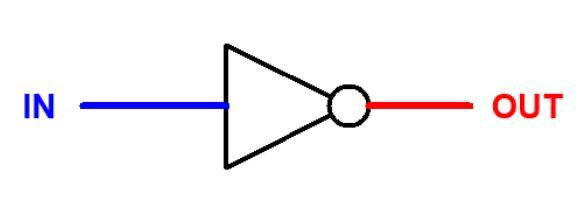
\includegraphics[width=0.5\linewidth]{images/not-gate}
    \caption{NOT gate}
    \label{fig:placeholder3}
\end{figure}

\begin{table}[H]
    \centering
    \caption*{\textbf{Truth Table: Inverter Gate}}
    \begin{tabular}{cc}
        \toprule
        $x$(IN) & $y$(OUT) \\
        \midrule
        0 & 1 \\
        1 & 0 \\
        \bottomrule
    \end{tabular}
\end{table}
 \begin{center}
 Boolean Expression: 
  x = y    
\end{center}

\subsection*{OR gate}

The OR gate that is true(1) when one or both inputs are true(1). If all OR gates are false, the output is false(0). The output is the Boolean sum of their values. The inputs are on the left and the outputs on the right.

\begin{figure}[H]
    \centering
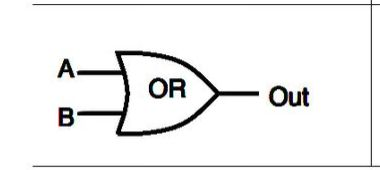
\includegraphics[width=0.5\linewidth]{images/or-gate}
    \caption{OR gate}
    \label{fig:placeholder4}
\end{figure}

\begin{table}[H]
    \centering
    \caption*{\textbf{Truth Table:OR Gate}}
    \begin{tabular}{ccc}
        \toprule
        $x$ & $y$ & $x + y$(out) \\
        \midrule
        0 & 0 & 0 \\
        1 & 0 & 1 \\
        0 & 1 & 1 \\
        1 & 1 & 1 \\
        \bottomrule
    \end{tabular}
\end{table}

\begin{center}
Boolean Expression: $A = x + y$
\end{center}

\subsection*{AND gate}

The  AND gate that is used to perform logical multiplication of input. The output of the AND gate will be true if both inputs are true(1), otherwise the output will be false(0) if any of the input is false(0). The input is shown on the left,and the output is shown on the right.

\begin{figure}[H]
    \centering
    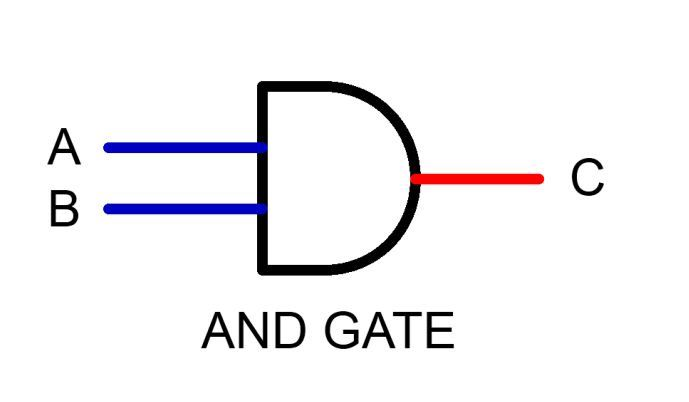
\includegraphics[width=0.5\linewidth]{images/and-gate}
    \caption{AND gate}
    \label{fig:placeholder5}
\end{figure}

\begin{table}[H]
    \centering
    \caption*{\textbf{Truth Table: AND Gate}}
    \begin{tabular}{ccc}
        \toprule
$a$ & $b$ & $a \cdot b$(c) \\
\midrule
0 & 0 & 0 \\
1 & 0 & 0 \\
0 & 1 & 0 \\
1 & 1 & 1 \\
        \bottomrule
    \end{tabular}
\end{table}

\begin{center}
Boolean Expression: $A$ = $a \cdot b$
\end{center} 

\subsection*{NAND gate}

The NAND gate, also known as negated AND, gives an output is false(0) if both inputs are true(1). The inputs are shown on the left,and the output is shown on the right.

\begin{figure}[H]
    \centering
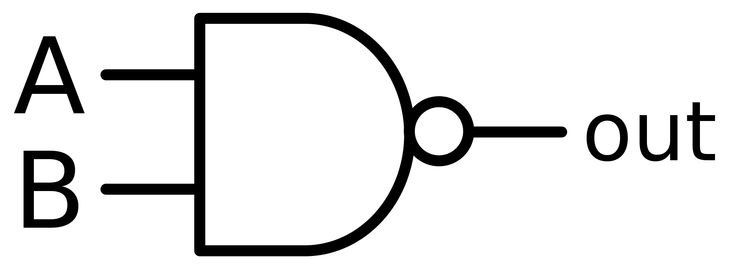
\includegraphics[width=0.5\linewidth]{images/nand-gate}
    \caption{NAND gate}
    \label{fig:placeholder6}
\end{figure}

\begin{table}[H]
    \centering
    \caption*{\textbf{Truth Table: NAND Gate}}
    \begin{tabular}{ccc}
        \toprule
  $a$ & $b$ & $\overline{ab}$'(c) \\
 \midrule
  0 & 0 & 1 \\
  0 & 1 & 1 \\
  1 & 0 & 1 \\
  1 & 1 & 0 \\
        \bottomrule
    \end{tabular}
\end{table}

\begin{center}
Boolean Expression: $A = \overline{x \cdot y}$
\end{center}

\subsection*{NOR gate}

A NOR gate is a digital circuit that gives us a true(1) output when there are false(0) input signals.

\begin{figure}[H]
    \centering
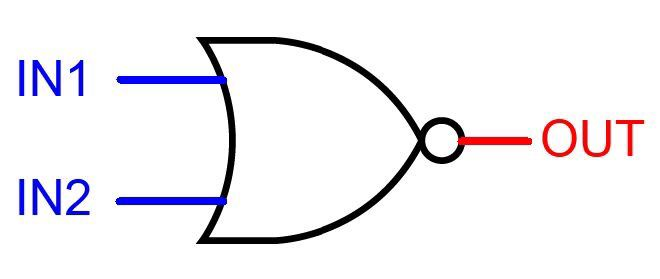
\includegraphics[width=0.5\linewidth]{images/nor-gate}
    \caption{NOR gate}
    \label{fig:placeholder7}
\end{figure}

\begin{table}[H]
    \centering
    \caption*{\textbf{Truth Table:NOR Gate}}
    \begin{tabular}{ccc}
        \toprule
         $x$ & $y$ & $\overline{x + y}$(out) \\
        \midrule
        0 & 0 & 1 \\
        0 & 1 & 0 \\
        1 & 0 & 0 \\
        1 & 1 & 0 \\
        \bottomrule
    \end{tabular}
\end{table}

\begin{center}
Boolean Expression: $A = \overline{x + y}$
\end{center}

\subsection*{XOR gate}

An XOR also known as Exclusive OR gate is a digital logic gate that outputs true(1) only when the number of inputs is odd.

\begin{figure}[H]
    \centering
    
\includegraphics[width=0.5\linewidth]{images/xor-gate}
    \caption{XOR gate}
    \label{fig:placeholder8}
\end{figure}

\begin{table}[H]
    \centering
    \caption*{\textbf{Truth Table:XOR Gate}}
    \begin{tabular}{ccc}
        \toprule
        $x$ & $y$ & $x \oplus y$(out) \\
        \midrule
        0 & 0 & 1 \\
        0 & 1 & 0 \\
        1 & 0 & 0 \\
        1 & 1 & 1\\
        \bottomrule
    \end{tabular}
\end{table}

\begin{center}
Boolean expression: $A = x \oplus y$
\end{center}

\subsection{Combinations of Gates}

Combinational circuits can be built using inverters, OR gates and, the AND gates at the same time, where some gates may share inputs; this can be shown by using branching line or written separately for each gate.

steps on how to make a combinational cirucUit;

\textbf {1.} Identify the inputs and outputs of the circuit.

\textbf{2.} Draw a truth table with all possible input values that should match the output values.

\textbf{3.} Derive the Boolean expression for the circuit.

\textbf{4.} Simplify the Boolean expression using K-Map or algebraic methods

\textbf{5.} Draw  the logic diagram using the Boolean expression

For example;

\begin{figure}[H]
    \centering
    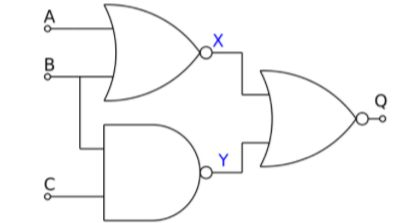
\includegraphics[width=0.5\linewidth]{images/combinational-circuit}
    \caption{Combinational circuit}
    \label{fig:placeholder9}
\end{figure}

\begin{table}[H]
    \centering
    \caption*{\textbf{Truth Table:Combinational circuit}}
    \begin{tabular}{ccccccc}
        \toprule
        $A$ & $B$ & $C$ & $X$ & $Y$ & $Z$ & $Q$\\
        \midrule
        0 & 0 & 0 & 0 & 1 & 1 & 0 \\
        0 & 0 & 1 & 0 & 1 & 1 & 0 \\
        0 & 1 & 0 & 1 & 0 & 0 & 0\\
        0 & 1 & 1 & 1 & 0 & 1 & 1\\
        1 & 0 & 0 & 1 & 1 & 1 & 1\\
        1 & 0 & 1 & 1 & 1 & 1 & 1\\
        1 & 1 & 0 & 1 & 0 & 0 & 0\\
        1 & 1 & 1 & 1 & 0 & 1 & 1\\
        \bottomrule
    \end{tabular}
\end{table}    


\newpage

\section{EXAMPLES OF CIRCUITS}


\subsection{DEFINITION}

A Circuit ( in a digital logic ) is a system made up of logic gates that processes input signals ( usually represented as 0s and 1s ) to produce an output based on a defined rule or function.
\\
Basically, circuits are designed to perform useful functions.. They take inputs (e.g x,y, and z) and produce an output using Boolean logic. The behavior of a circuit can be described using a Boolean expression.

\subsection{Examples}

The following are some examples of circuits and their solutions.


\subsection{EXAMPLE 1}
 A committee of three individuals decides on issues for an organization. Each individual vote yes or no for each proposal that arises. A proposal is passed if it receives at least two yes votes. Design a circuit that determines whether a proposal passes.

\textbf{Solution:}
Let $x=1$ if the first individual votes yes and $x=0$ if this individual votes no; let $y=1$ if the second individual votes yes and $y=0$ if this individual votes no; let $z=1$ if the third individual votes yes and $z=0$ if this individual votes no. Then a circuit must be designed that produces the output 1 when two or more of $x,y,z$ are 1. One Boolean expression for this is
\[
xy+xz+yz.
\]
\begin{figure}[H]
    \centering
    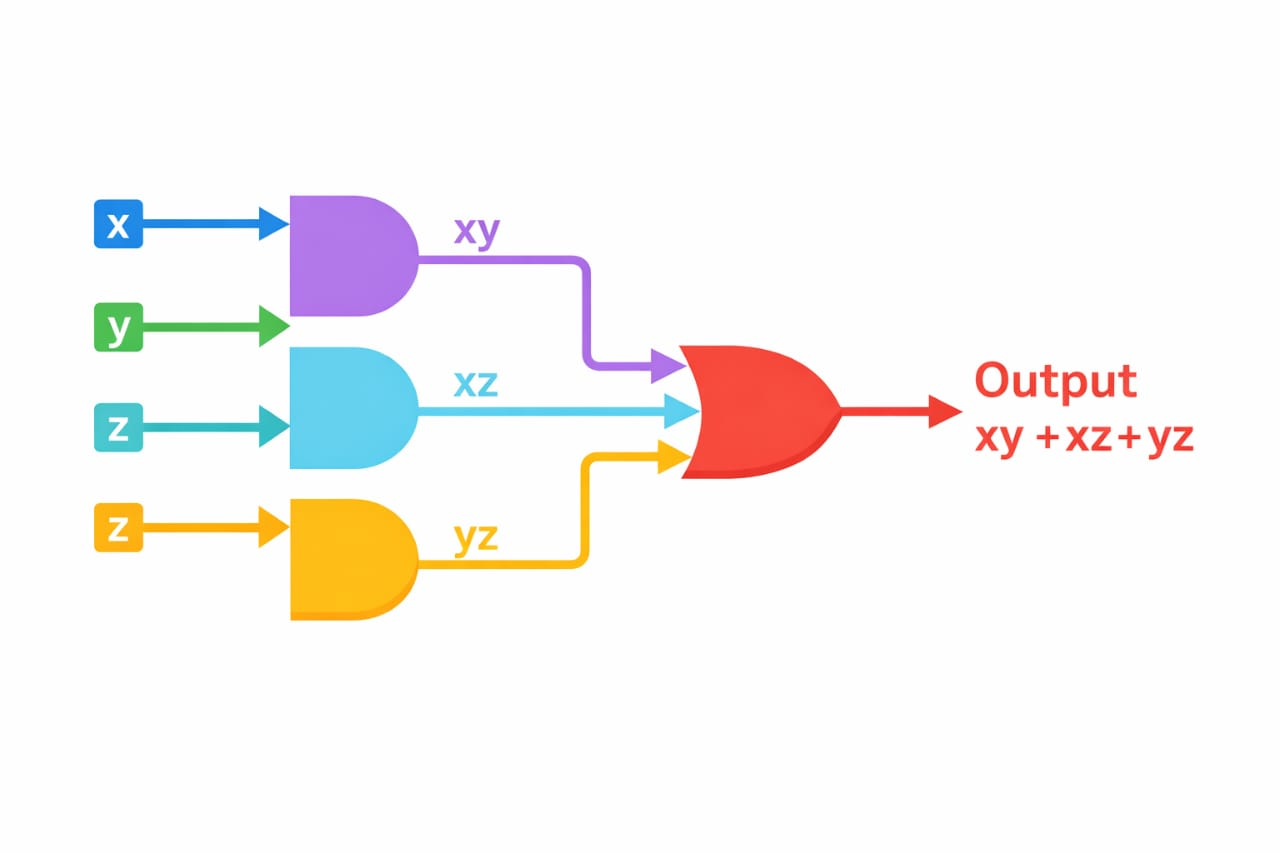
\includegraphics[width=0.75\linewidth]{WhatsApp Image 2026-04-13 at 20.37.12.jpeg}
    \caption{Figure 5: A circuit for Majority Voting}
    \label{fig:placeholder}
\end{figure}

\subsection{EXAMPLE 2}

Sometimes light fixtures are controlled by more than one switch. Circuits need to be designed so that flipping any one of the switches for the fixture turns the light on when it is off and turns the light off when it is on. Design circuits that accomplish this when there are two switches and when there are three switches.

   \textbf{Solution:}
 We begin by designing the circuit that controls the light fixture when two different switches are used. Let $x=1$ when the first switch is closed and $x=0$ when it is open and let $y=1$ when the second switch is closed and $y=0$ when it is open. Let $F(x,y)=1$ when the light is on and $F(x,y)=0$ when it is off. We can arbitrarily decide that the light will be on when both switches are closed, so that $F(1,1)=1$. This determines the remaining values:



\begin{figure}[H]
    \centering
    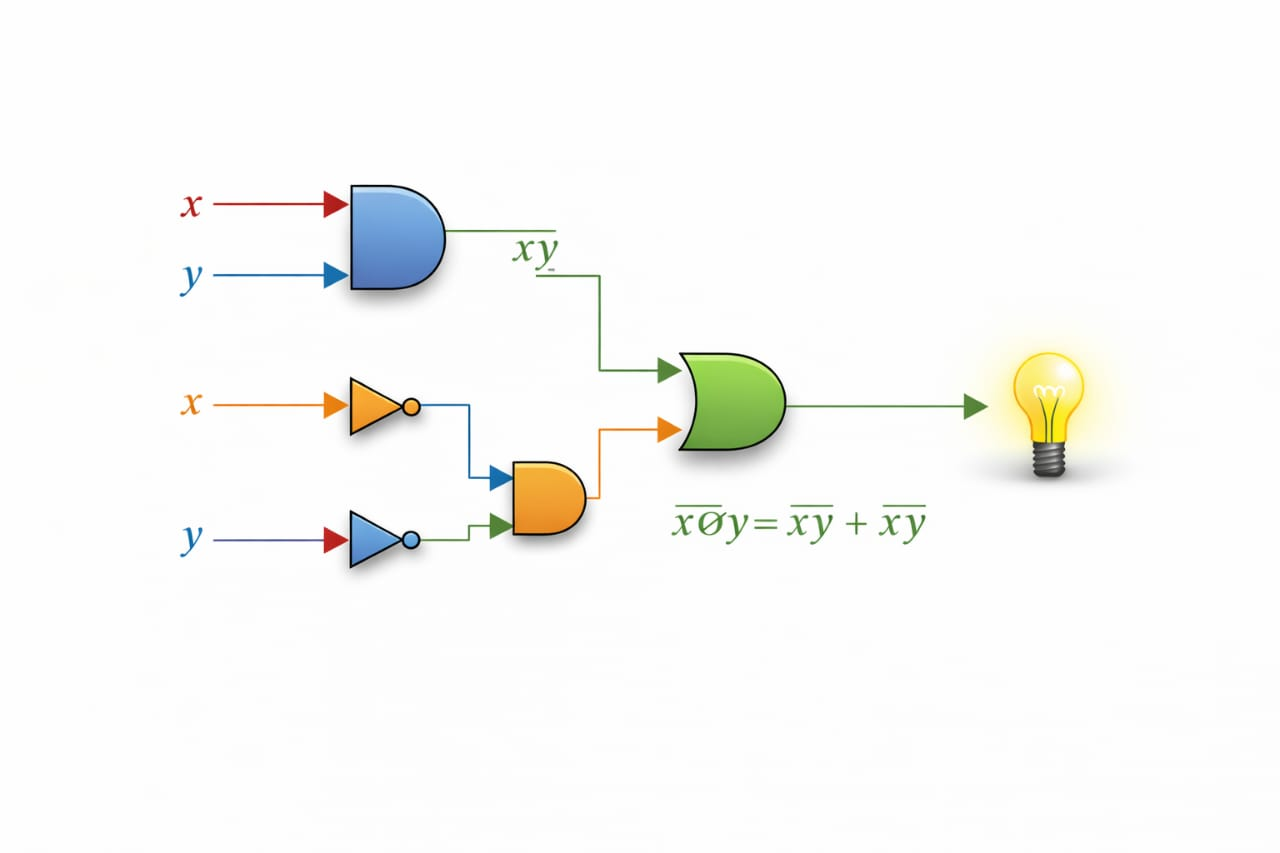
\includegraphics[width=0.75\linewidth]{image.png}
    \caption{Enter Caption}
    \label{fig:placeholder}
\end{figure}


\section*{{ADDERS}}

An adder is a digital logic circuit in electronices that implement the addition of numbers.
Half adder: is a combinational circuit that performs the addition of two bits, this circuit needs two binary inputs and two binary outputs.
Adding two single-bit binary values, X and Y produces a sum S bit and a carryout C-out bit.





\textbf{TABLE 3: Input and Output for the Half Adder}

\[
\begin{array}{|c|c||c|c|}
\hline
\multicolumn{2}{|c||}{\textbf{Input}} & \multicolumn{2}{c|}{\textbf{Output}} \\
\hline
x & y & s & c \\
\hline
1 & 1 & 0 & 1 \\
\hline
1 & 0 & 1 & 0 \\
\hline
0 & 1 & 1 & 0 \\
\hline
0 & 0 & 0 & 0 \\
\hline
\end{array}
\]

\vspace{0.5cm}



\begin{figure}[H]
    \centering
    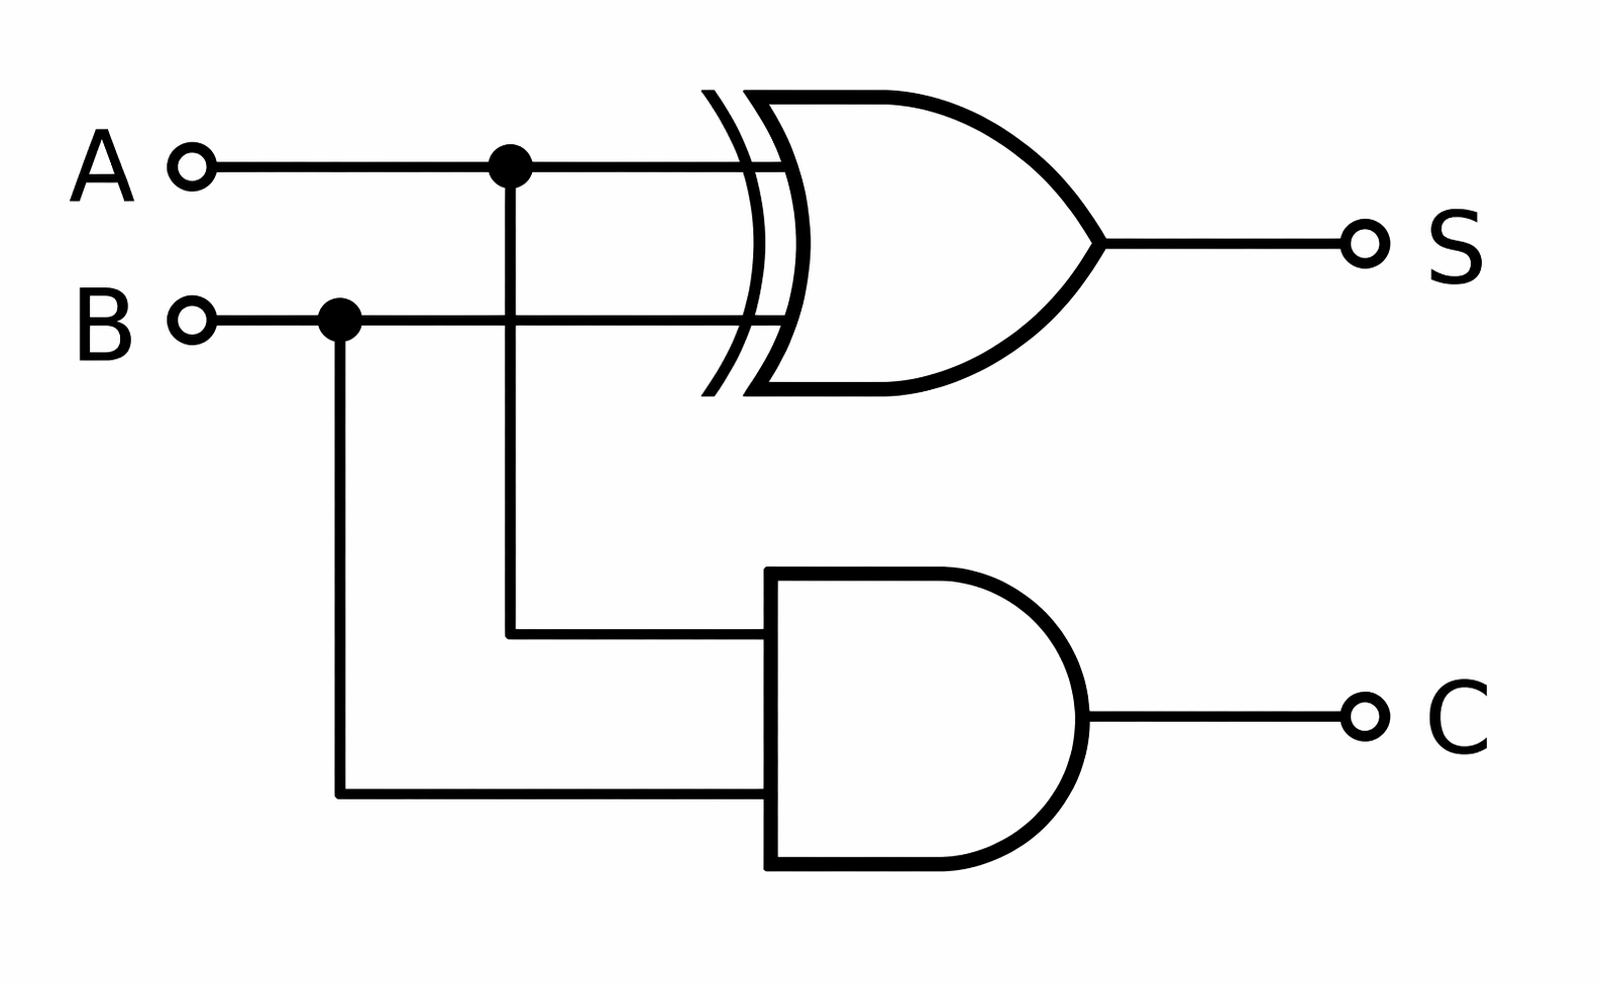
\includegraphics[width=0.6\textwidth]{images/image.png}
    \caption{FIGURE 7: The Half Adder}
    \label{fig:half_adder}
\end{figure}


\section* {Full Adder}

A full adder is a combinational circuit that performs the addition of three bits (two significant bits and a previous carry).
.it consists of three outputs and two outputs, where two inputs are the bits to be added , the third input represent the carry from the previous position.
. Adding two single-bit binary values Xand Y with a carry input bit C-in produces a sum bit Sand a carry out C-out bit.

 The Boolean expressions for the full adder are
\[
s = xyc_i + x\bar{y}\bar{c_i} + \bar{x}y\bar{c_i} + \bar{x}\bar{y}c_i
\]
and
\[
c_{i+1} = xyc_i + xy\bar{c_i} + x\bar{y}c_i + \bar{x}yc_i.
\]
These expressions account for all possible combinations of the three inputs and ensure that the correct sum and carry values are produced. The full adder is more powerful than the half adder because it allows the inclusion of carry propagation, which is essential for performing addition on numbers with more than one bit.

\begin{center}
\textbf{{TABLE 4}}\\[0.2cm]
\textbf{Input and Output for the Full Adder}
\[
\begin{array}{|c|c|c||c|c|}
\hline
\multicolumn{3}{|c||}{\textbf{Input}} & \multicolumn{2}{c|}{\textbf{Output}}\\
\hline
x & y & c_i & s & c_{i+1} \\
\hline
0 & 0 & 0 & 0 & 0 \\
\hline
0 & 0 & 1 & 1 & 0 \\
\hline
0 & 1 & 0 & 1 & 0 \\
\hline
0 & 1 & 1 & 0 & 1 \\
\hline
1 & 0 & 0 & 1 & 0 \\
\hline
1 & 0 & 1 & 0 & 1 \\
\hline
1 & 1 & 0 & 0 & 1 \\
\hline
1 & 1 & 1 & 1 & 1 \\
\hline
\end{array}
\]
\end{center}


\begin{figure}[H]
    \centering
    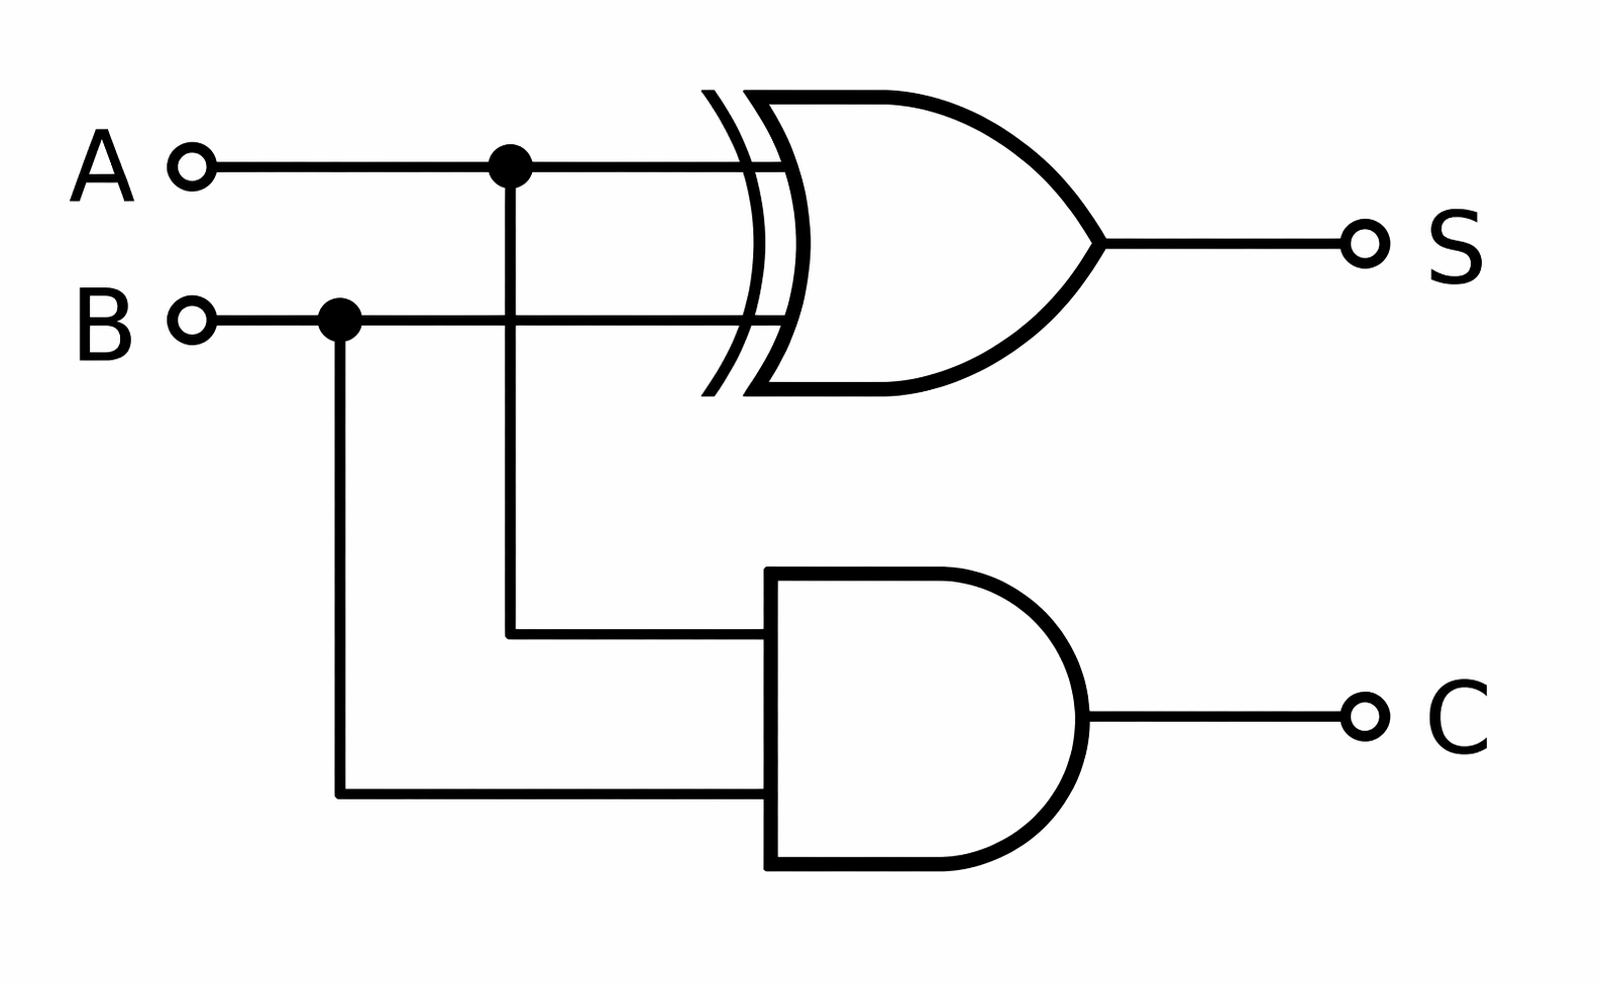
\includegraphics[width=0.7\textwidth]{images/image.png}
    \caption{FIGURE 8: The Full Adder}
    \label{fig:full_adder}
\end{figure}


\section{EXCERCISES}

\textbf{1.} Design a circuit that implements majority voting for five individuals.

\vspace{0.3cm}

\textbf{2.} Design a circuit for a light fixture controlled by four switches, where flipping one of the switches turns the light on when it is off and turns it off when it is on.

\vspace{0.3cm}

\textbf{3.} Show how the sum of two five-bit integers can be found using full and half adders.

\vspace{0.3cm}





\textbf{4.} Construct a circuit that compares the two-bit integers $(x_1x_0)_2$ and $(y_1y_0)_2$, returning an output of 1 when the first of these numbers is larger and an output of 0 otherwise.

\vspace{0.3cm}




\newpage
\section{Circuit Minimization}

\subsection{Why Minimization Matters}

\subsection{Minimization Techniques}

\subsection{Complexity of Boolean Minimization}

%\subsection*{Karnaugh Maps (K-Maps)}

%Karnaugh maps are used to minimize Boolean expressions, which helps in designing simpler digital circuits. Minimizing circuits is important because it reduces the number of logic gates required, leading to lower cost, less power consumption, and faster operation due to reduced delay. This makes the overall system more efficient and reliable.

%\subsubsection*{Steps to Use K-Maps}

%\textbf{Step 1: Choose the K-map} \\
%Select the correct K-map based on the number of variables (e.g., 2, 3, or 4 variables).

%\textbf{Step 2: Identify minterms or maxterms} \\
%Determine which combinations of inputs produce a 1 (minterms) or 0 (maxterms) from the given function.

%\textbf{Step 3: Fill in the K-map} \\
%For SOP, place 1s in the cells corresponding to the minterms and 0s elsewhere.

%\textbf{Step 4: Form groups} \\
%Group adjacent cells containing 1s. Each group must have a size that is a power of 2 (e.g., 2, 4, 8).

%\textbf{Step 5: Follow grouping rules} \\
%Groups must be as large as possible, no diagonal grouping is allowed, overlapping is allowed, and wrapping around edges is permitted.

%\textbf{Step 6: Derive simplified terms} \\
%For each group, identify the variables that remain constant and eliminate those that change.

%\textbf{Step 7: Write the final expression} \\
%Combine all simplified terms to form the minimized Boolean expression.

%\subsubsection*{Example}

%Given $F(A, B) = \Sigma m(0,1)$, place 1s in the cells for $m_0$ and $m_1$. These two cells are adjacent, so they form a group of 2.

%$B$ changes, so it is eliminated, and $A$ remains constant at 0.

%Final simplified expression:
%\[
%F = \overline{A}
%\]

\newpage
\section{Don't Care Conditions}

\subsection{Definition}
A don't care condition occurs when the output of a logic circuit for a
specific input combination is irrelevant. These inputs are represented by \textit{d}
in Karnaugh-maps. Other representations that can be used are X, $\phi$
or $-$, these are commonly used in truth tables.

\subsection{Why They Arise}

Don't care conditions typically arise in two situations:

\begin{description}
    \item[Invalid input combinations.] In a BCD (Binary Coded Decimal)
    system, only the input combinations \(0000\) to \(1001\) (representing
    digits 0--9) are valid. The remaining six combinations (\(1010\) to
    \(1111\)) can never occur, so their outputs are assigned as don't cares.

    \item[Unused outputs.] In some systems a particular input state is
    reachable, but the resulting output is never used by any other part of
    the circuit, making it irrelevant to the designer.
\end{description}

\subsection{How They Are Used}

During minimisation, don't care entries may be treated as either 0 or 1 —
whichever choice produces the simplest expression. This gives the designer
freedom to form \textbf{larger groupings (implicants)}, which directly
reduces the number of logic gates in the final circuit. A key rule applies:
a grouping may \emph{include} don't cares to enlarge it, but it cannot
consist \emph{entirely} of don't cares, as such a group covers no required
output.

\subsection{Truth Table Example}

Consider the function \(f(A,B,C) = \sum m(1,3,7) + \sum d(2,5)\), shown
in Table~\ref{tab:dontcare}. Minterms 2 and 5 are don't cares and can be
included in groupings during minimisation to yield a simpler final
expression.

\begin{table}[h!]
\centering
\caption{Truth table with don't care conditions}
\label{tab:dontcare}
\begin{tabular}{@{}ccccc@{}}
\toprule
\textbf{Minterm} & \textbf{A} & \textbf{B} & \textbf{C} &
\textbf{Output} \\
\midrule
0 & 0 & 0 & 0 & 0 \\
1 & 0 & 0 & 1 & 1 \\
2 & 0 & 1 & 0 & \(d\) \\
3 & 0 & 1 & 1 & 1 \\
4 & 1 & 0 & 0 & 0 \\
5 & 1 & 0 & 1 & \(d\) \\
6 & 1 & 1 & 0 & 0 \\
7 & 1 & 1 & 1 & 1 \\
\bottomrule
\end{tabular}
\end{table}


\section{Quine-McCluskey Method}

\subsection{Definition}
The Quine-McCluskey method is a tabular, algorithmic approach to Boolean
function minimisation. It is essentially a more systematic and
computer friendly version of the Karnaugh map method. This method is a
deterministic algorithm that can be programmed and is effective for any
number of variables.

\subsubsection{How It Works}

The Quine-McCluskey method proceeds in two well-defined stages.

\begin{description}
    \item[Step 1: Finding prime implicants.]
    This step identifies the largest possible groups of 1s and don't cares
    that can be combined. It works by first listing all minterms and don't
    cares in binary and sorting them into groups according to the number of
    1-bits in their binary representation. Terms from adjacent groups are
    then compared and merged if they differ in exactly one bit
    position, using the algebraic identity:
    \[
        AB + AB' = A
    \]
    The differing bit is replaced with a dash ($-$) to indicate elimination.
    This process repeats on the resulting terms until no further merging is
    possible. Any term that cannot be merged further is a prime implicant.

    \item[Step 2: Finding the essential prime implicants.]
    This step selects the minimal set of prime implicants needed to cover
    all the original minterms, the 1s of the function. A
    prime implicant chart is constructed with prime implicants as
    rows and original minterms as columns. A prime implicant is
    essential if it is the only one covering a particular minterm, it must be included in the final expression. After selecting all
    essential prime implicants, any uncovered minterms are resolved by
    choosing additional prime implicants, preferring those that cover the
    most remaining minterms. This is a classic set-covering problem.
\end{description}

\subsubsection{Example}

Given: \(f(A,B,C,D) = \sum m(0,1,2,5,6,7,8,9,10,14)\)

All minterms are listed in binary and sorted by their number of 1 bits,
as shown in Table~\ref{tab:grouping}. Adjacent groups are then compared and
combined where possible, producing the first-round combinations in
Table~\ref{tab:combinations}.Combining continues on these results until no further merging is possible.
Terms that remain uncombined are the prime implicants. These are entered
into the prime implicant chart, essential prime implicants are identified,
and the minimised Sum of Products expression is written.

\begin{table}[h!]
\centering
\caption{Minterms grouped by number of 1-bits}
\label{tab:grouping}
\begin{tabular}{@{}ccc@{}}
\toprule
\textbf{\# of 1s} & \textbf{Minterm} & \textbf{A\;B\;C\;D} \\
\midrule
0 & 0  & 0\;0\;0\;0 \\
\midrule
1 & 1  & 0\;0\;0\;1 \\
  & 2  & 0\;0\;1\;0 \\
  & 8  & 1\;0\;0\;0 \\
\midrule
2 & 5  & 0\;1\;0\;1 \\
  & 6  & 0\;1\;1\;0 \\
  & 9  & 1\;0\;0\;1 \\
  & 10 & 1\;0\;1\;0 \\
\midrule
3 & 7  & 0\;1\;1\;1 \\
  & 14 & 1\;1\;1\;0 \\
\bottomrule
\end{tabular}
\end{table}

\begin{table}[h!]
\centering
\caption{First-round combinations}
\label{tab:combinations}
\begin{tabular}{@{}lll@{}}
\toprule
\textbf{Minterms} & \textbf{Result} & \textbf{A\;B\;C\;D} \\
\midrule
0,\;1   & (0,1)  & 0\;0\;0\;-- \\
0,\;2   & (0,2)  & 0\;0\;--\;0 \\
0,\;8   & (0,8)  & --\;0\;0\;0 \\
1,\;9   & (1,9)  & --\;0\;0\;1 \\
2,\;6   & (2,6)  & 0\;--\;1\;0 \\
2,\;10  & (2,10) & --\;0\;1\;0 \\
8,\;9   & (8,9)  & 1\;0\;0\;-- \\
8,\;10  & (8,10) & 1\;0\;--\;0 \\
6,\;7   & (6,7)  & 0\;1\;1\;-- \\
6,\;14  & (6,14) & --\;1\;1\;0 \\
\bottomrule
\end{tabular}
\end{table}


\newpage
\bibliographystyle{ieeetr}
\bibliography{references}

\end{document}
